\documentclass[11pt]{scrartcl}


\usepackage{amsmath,amsthm,amssymb}
\usepackage{hyperref}
\usepackage{mathtools}
\usepackage{enumerate}
\usepackage{graphicx}
\usepackage{mathpazo}
\usepackage{lmodern}
\usepackage{parskip}

\theoremstyle{plain} 
\newtheorem{theorem}{Theorem}
\newtheorem{lemma}[theorem]{Lemma}
\newtheorem{algorithm}{Algorithm}
\DeclarePairedDelimiter\ceil{\lceil}{\rceil}
\DeclarePairedDelimiter\floor{\lfloor}{\rfloor}


\theoremstyle{definition}
\newtheorem*{definition}{Definition} 
\theoremstyle{remark}
\newtheorem{remark}{Remark}


\usepackage[margin=1in]{geometry}

\usepackage{fancyhdr}
\pagestyle{fancy}
\lhead{15-418 Writeup}
\rhead{Jacob Imola (jimola), Sidhanth Mohanty (smohant1)} 
\cfoot{\thepage}

\DeclareMathOperator{\Tr}{\mathsf{Tr}}

\newcommand{\half}{\frac{1}{2}}
\newcommand{\cbrt}[1]{\sqrt[3]{#1}}
\newcommand{\Prob}{\textbf{Pr}}
\newcommand{\eps}{\varepsilon}
\newcommand{\E}{\textbf{E}}
\newcommand{\Ind}{\boldsymbol{1}}
\newcommand{\Ener}{\mathcal{E}}
\newcommand{\Var}{\textbf{Var}}
\newcommand{\rank}{\mathsf{rank}}

\begin{document}

\title{15-418 Project Proposal: Parallel Low Diameter Decompositions in Graphs}
\author{\textsf{Jacob Imola (jimola), Sidhanth Mohanty (smohant1)}}
\date{\textsf{\today}}
\maketitle

\section{Summary}
We implemented an algorithm from a paper of Gary Miller, Richard Peng and Shen Xu \cite{miller2013parallel}
to perform a low diameter decomposition in graphs in parallel using \texttt{C++} and \texttt{OpenMP}.
Depending on the structure of the graph, we achieved somewhere between a $2$-$3\times$ when using all
the cores on a single machine in \texttt{latedays} compared to the single threaded implementation of
this algorithm. We also implemented a work efficient simple sequential algorithm, and unfortunately,
on some sparse graphs, the sequential algorithm is more efficient.

\section{Background}
A low diameter decomposition of a graph is a partition of the vertices of the graph into clusters such
that the distance between any two vertices inside a single cluster is small and the number of edges
between any two clusters is small compared to the total number of internal edges. Formally, an $(\alpha,
\beta)$ LDD of the graph is a decomposition of $V$ into disjoint $V_1,V_2,\ldots,V_t$ such that for
any $v_1,v_2\in V_i$, $d(v_1,v_2)\leq\alpha$ and the number of edges leaving $V_i$ is at least a
$\beta$ fraction of the number of internal edges in $V_i$.

The baseline sequential algorithm to find a $(\frac{\log n}{\beta},\beta)$-LDD works in the following way:
pick a vertex and start a BFS and stop when the fraction of edges leaving the current component is less
than $\beta(\text{number of internal edges})$. Put all the visited vertices in a cluster and recurse on the
remaining graph.

The reason this algorithm is not nicely parallelizable is that picking clusters is an inherently sequential process.
Miller-Peng-Xu \cite{miller2013parallel} propose an algorithm to bypass this limitation, which we describe below:

\begin{enumerate}

\item Assign a value $\delta_u\sim\text{Exp}(\beta)$ to each vertex $u$ (a parallel step). This value is the amount of ``head start'' that each vertex gets.

\item Compute $\delta_{\text{max}} = \max\{\delta_u|u\in V\}$, and set the start times of vertex $u$ as $\delta_{\text{max}}-\delta_u$.

\item Do a single BFS, where each vertex in the frontier belongs to a cluster and set any neighbors in the next frontier to the same cluster. Each round of BFS takes 1 second, and a vertex $v$ with start time $S$ joins the frontier at round $\lfloor S \rfloor$ with its own cluster if it hasn't already been visited. We store $S-\lfloor S \rfloor$ as a tie-breaker; if a vertex $u$ in the next frontier hit by multiple vertices in the current frontier, $u$ belongs to the smallest cluster. It is not hard to see that a vertex will belong to the cluster of the vertex that has the minimum distance minus head start.

\end{enumerate}
Steps 1 and 2 are extremely parallelizable. Step 3 involves a single BFS, so it's parallelization depends on the topology of the graph. For each vertex, we store the cluster it belongs to and its minimum tiebreaker.
Multiple BFS's happening in parallel causes multiple clusters to form at once and is the key step in
achieving parallelism. We note that for smaller values of
$\beta$ the performance of the parallel algorithm worsens
but the sequential algorithm runs in exactly the same
amount of time. Also, the parallel algorithm is more
complicated and hence a sequential version of it is
slower than the sequential baseline that we have.

\section{The Approach}
We used \texttt{C++} with \texttt{OpenMP} and optimized our code on the \texttt{latedays} machine.

\begin{itemize}
\item In the first step of assigning a value to each vertex,
we run a \texttt{\#pragma omp parallel for} loop to
have multiple threads assign values to different vertices
at the same time.

\item Although the max can be computed using a reduce, we do
it sequentially since the advantage of reduce is noticable
only in a large number of cores.

\item Constructing the new frontier from the old frontier
can be done in parallel by having different threads
retrieve a list of neighbors of different vertices
in the frontier, then these different lists are merged
to get the new frontier. We were initially using
a standard \texttt{OpenMP \#pragma omp parallel for}
loop and then later added dynamic scheduling, and we noticed
a speedup.

\end{itemize}

We spent some time optimizing our simple sequential
baseline to make sure that our parallel implementation
was being compared against a fair test harness.
In our initial sequential version, we were adding
all neighbors to a tentative frontier (with possible
duplicates because we didn't want to assign vertices
to clusters before making sure that there were enough
edges leaving the current cluster) and then going
through this fully created list to count the number
of edges and process the new frontier (without
duplicates). Running this code on dense graphs
completely killed performance so we modified our
code to not store duplicates. We were also
storing 2 arrays whose $i$th element was accessed
at similar times, and then got a minor speedup
with better cache locality by having one array
of length $2n$ where even indices store one array
and odd indices store the other array.

We didn't use any existing pieces of code and started from
scratch.

\section{Results}

<insert bunch of results here, and graphs>

There was still more scope for parallelism and all the
CPU cores did not exhaust the opportunities for parallelism.
Indeed, the strength of the parallel algorithm was that
it had very good span and hence would benefit from
more cores, and hence doing the project using CUDA
on a Nvidia GPU instead of using \texttt{OpenMP} might have
been a better idea.
\begin{figure}
\vspace*{-3cm}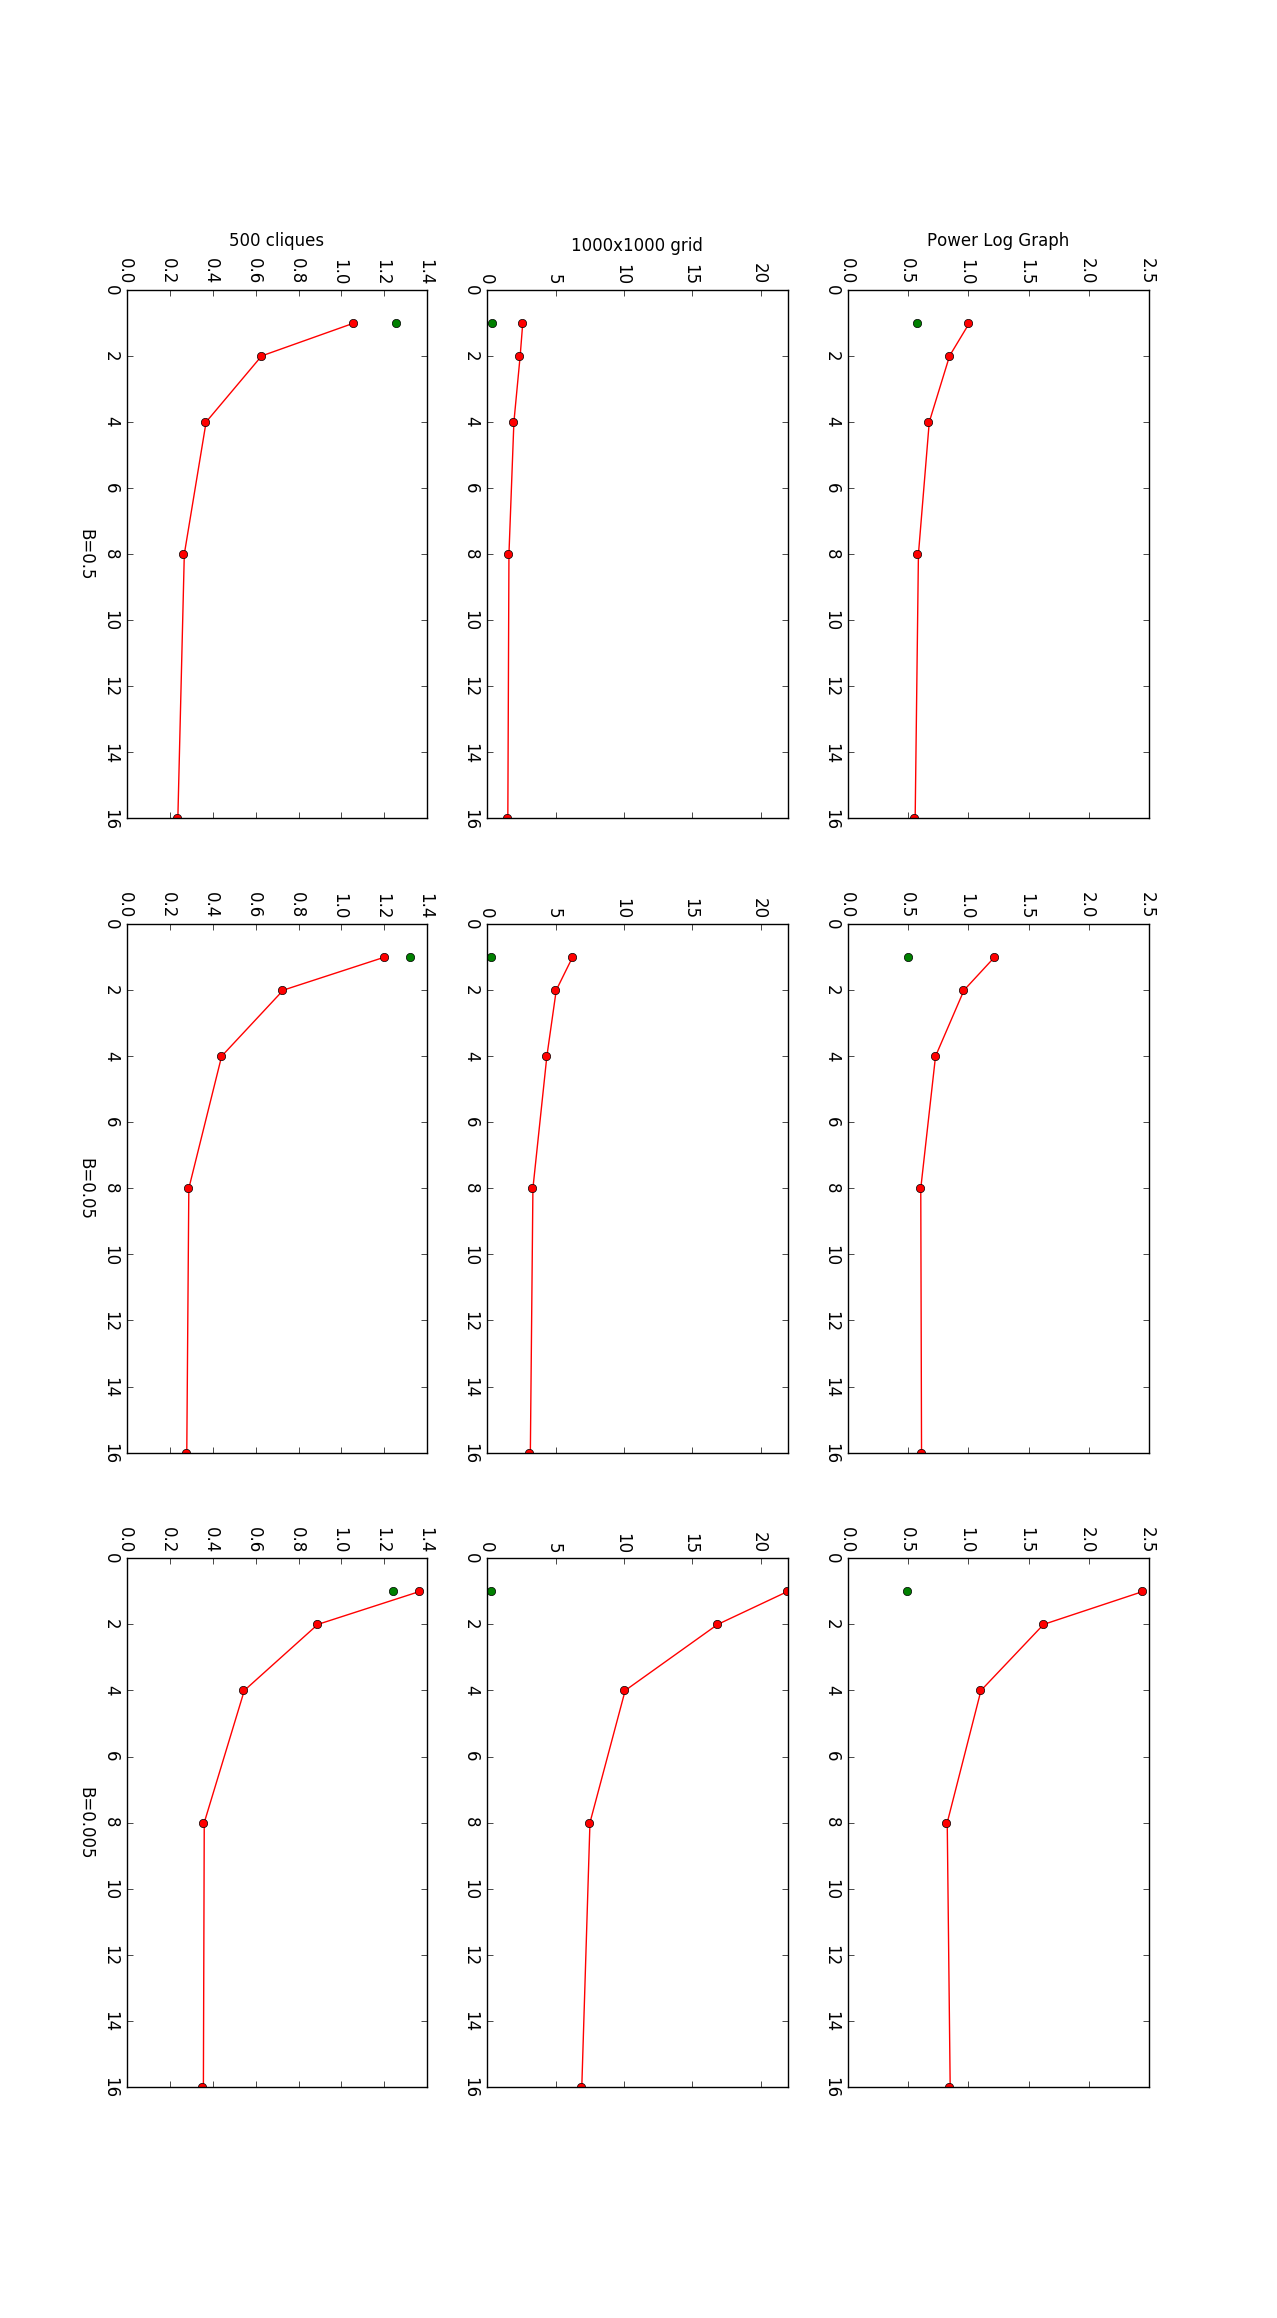
\includegraphics[width=\textwidth]{Speedup_plots.png}\vspace{-3cm}
\caption{Speedup plots for 3 different graphs and 3 different values of $\beta$.}
\end{figure}
\section{List of work by each student}
\begin{itemize}

\item \textbf{Jacob:} Implemented the Miller-Peng-Xu
algorithm and parallelized it in OpenMP, also optimized
and improved the sequential baseline written by Sidhanth.
Also wrote the setup code in \texttt{main.cpp}.

\item \textbf{Sidhanth:} Wrote the sequential baseline and
performed some optimizations on the MPX algorithm.

\end{itemize}

\bibliographystyle{alpha}
\bibliography{project_proposal}

\end{document}
